\documentclass[portrait,final,a0paper]{baposter}
%\documentclass[a4shrink,portrait,final]{baposter}
% Usa a4shrink for an a4 sized paper.

\tracingstats=2

% special 
\usepackage{ifthen}
\usepackage{ifpdf}
\usepackage{float}
\usepackage{color}

% fonts
\usepackage{latexsym}
\usepackage{amsmath} 
\usepackage{amssymb} 
\usepackage{bm}
\usepackage{wasysym}


\ifpdf
\usepackage{graphicx}
\usepackage{epstopdf}
\else
\usepackage{graphicx}
\usepackage{epsfig}
\fi


\graphicspath{{figures/},{PROG/figures/}}


%%%%%%%%%%%%%%%%%%%%%%%%%%%%%%%%%%%%%%%%%%%%%%%%%%%%%%%%%%%%%%%%


% NEW 
\newcommand{\abs}[1]{\left|#1\right|}
\newcommand{\Prob}{\mbox{Prob}\,}
\newcommand{\erf}{\mbox{erf}\,}
\newcommand{\barline}[1]{#1}

% math symbols I
\newcommand{\sinc}{\mbox{sinc}}
\newcommand{\const}{\mbox{const}}
\newcommand{\trc}{\mbox{trace}}
\newcommand{\intt}{\int\!\!\!\!\int }
\newcommand{\ointt}{\int\!\!\!\!\int\!\!\!\!\!\circ\ }
\newcommand{\ar}{\mathsf r}
\newcommand{\im}{\mbox{Im}}
\newcommand{\re}{\mbox{Re}}

% math symbols II
\newcommand{\eexp}{\mbox{e}^}
\newcommand{\bra}{\left\langle}
\newcommand{\ket}{\right\rangle}

% Mass symbol
\newcommand{\mass}{\mathsf{m}} 
\newcommand{\Mass}{\mathsf{M}} 

% more math commands
\newcommand{\tbox}[1]{\mbox{\tiny #1}}
\newcommand{\bmsf}[1]{\bm{\mathsf{#1}}} 
%\newcommand{\amatrix}[1]{\matrix{#1}} 
\newcommand{\amatrix}[1]{\begin{matrix} #1 \end{matrix}} 
\newcommand{\pd}[2]{\frac{\partial #1}{\partial #2}}

% equations
\newcommand{\mylabel}[1]{\label{#1}} 
%\newcommand{\mylabel}[1]{\textcolor{blue}{[#1]}\label{#1}} 
\newcommand{\beq}{\begin{eqnarray}}
\newcommand{\eeq}{\end{eqnarray}} 
\newcommand{\be}[1]{\begin{eqnarray}\ifthenelse{#1=-1}{\nonumber}{\ifthenelse{#1=0}{}{\mylabel{e#1}}}}
\newcommand{\ee}{\end{eqnarray}} 

% arrangement
\newcommand{\drawline}{\begin{picture}(500,1)\line(1,0){500}\end{picture}}
\newcommand{\bitem}{$\bullet$ \ \ \ }
\newcommand{\Cn}[1]{\begin{center} #1 \end{center}}
\newcommand{\mpg}[2][1.0\hsize]{\begin{minipage}[b]{#1}{#2}\end{minipage}}
\newcommand{\mpgt}[2][1.0\hsize]{\begin{minipage}[t]{#1}{#2}\end{minipage}}
\newcommand{\putgraph}[2][width=0.30\hsize]{\includegraphics[#1]{#2}}

% more
%\newcommand{\Eq}[1]{Eq.\!\!~(\ref{#1})}
%\newcommand{\Fig}[1]{Fig.\!\!~\ref{#1}}  
\newcommand{\Eq}[1]{\textcolor{blue}{Eq.\!\!~(\ref{#1})}} 
\newcommand{\Fig}[1]{\textcolor{blue}{Fig.}\!\!~\ref{#1}} 
\newcommand{\hide}[1]{} %{\textcolor{red}{[hidden text]}} %{}
\newcommand{\rmrk}[1]{\textcolor{red}{#1}}


%%%%%%%%%%%%%%%%%%%%%%%%%%%%%%%%%%%%%%%%%%%%%%%%%%%%%%%%%%%%%%%%%%%%%%%%%%%

% extra math commands by jarondl
\newcommand{\inner}[2]{\left \langle #1 \middle| #2\right\rangle} % Inner product
\newcommand{\avgangle}[1]{\left\langle #1 \right\rangle} % Average <x>

%fminipage using fancybox package
\newenvironment{fminipage}%
  {\begin{Sbox}\begin{minipage}}%
  {\end{minipage}\end{Sbox}\fbox{\TheSbox}}

%%%%% REMOVING the bibliography title
\renewcommand{\refname}{}
    

%%%%%%%%%%%%%%%%%%%%%%%%%%%%%%%%%%%%%%%%%%%%%%%%%%%%%%%%%%%%%%%%%%%%%%%%%%%%%%
%%% Begin of Document
%%%%%%%%%%%%%%%%%%%%%%%%%%%%%%%%%%%%%%%%%%%%%%%%%%%%%%%%%%%%%%%%%%%%%%%%%%%%%%

\begin{document}

%%%%%%%%%%%%%%%%%%%%%%%%%%%%%%%%%%%%%%%%%%%%%%%%%%%%%%%%%%%%%%%%%%%%%%%%%%%%%%
%%% Here starts the poster
%%%---------------------------------------------------------------------------
%%% Format it to your taste with the options
%%%%%%%%%%%%%%%%%%%%%%%%%%%%%%%%%%%%%%%%%%%%%%%%%%%%%%%%%%%%%%%%%%%%%%%%%%%%%%
% Define some colors
\definecolor{silver}{cmyk}{0,0,0,0.3}
\definecolor{yellow}{cmyk}{0,0,0.9,0.0}
\definecolor{reddishyellow}{cmyk}{0,0.22,1.0,0.0}
\definecolor{black}{cmyk}{0,0,0.0,1.0}
\definecolor{darkYellow}{cmyk}{0,0,1.0,0.5}
\definecolor{darkSilver}{cmyk}{0,0,0,0.1}

\definecolor{lightyellow}{cmyk}{0,0,0.3,0.0}
\definecolor{lighteryellow}{cmyk}{0,0,0.1,0.0}
\definecolor{lighteryellow}{cmyk}{0,0,0.1,0.0}
\definecolor{lightestyellow}{cmyk}{0,0,0.05,0.0}

%%
%\background{
%  \begin{tikzpicture}[remember picture,overlay]%
%    \draw (current page.north west)+(-2em,2em) node[anchor=north west] {\includegraphics[height=1.1\textheight]{silhouettes_background}};
%  \end{tikzpicture}%
%}
\typeout{Poster Starts}



\begin{poster}%
  % Poster Options
  {
  bgColorOne=lightgray!30,
  %bgColorTwo=yellow,
  headerheight=0.1\textheight,
  columns=3,
  headershade=plain,
  headerColorOne=green!40,
  boxColorOne=lightgray!75,
  headershape=smallrounded,
  textborder=roundedsmall,
  linewidth=0.5pt,
  borderColor=green,
  headerborder=open,
  eyecatcher=false,
  background=plain
}
  % Eye Catcher
  {\includegraphics[width=10em]{D1077}} % No eye catcher for this poster. (eyecatcher=no above). If an eye catcher is present, the title is centered between eye-catcher and logo.
  % Title
  {\bf \vspace{1em}\center{
Transport in "sparse" networks:\\ 
\hspace{1em}From linear response to effective range hopping.}}
  % Authors
  {\sf
  \vspace{-1.2em}  {\center{Yaron de Leeuw, Doron Cohen\\
Ben-Gurion University of the Negev\\}}
%                Physics Department \\
%                 Ben-Gurion University of the Negev, \\
%                Beer-Sheva, Israel\\
%                \texttt{jarondl@bgu.ac.il}}
  }
  % University logo
  {\hspace{1em}
\includegraphics[height=10em]{BGU}\
  }

  \tikzstyle{light shaded}=[top color=baposterBGtwo!30!white,bottom color=baposterBGone!30!white,shading=axis,shading angle=30]


%%%%%%%%%%%%%%%%%%%%%%%%%%%%%%%%%%%%%%%%%%%%%%%%%%%%%%%%%%%%%%%%%%%%%%%%%%%%%%
%%% Now define the boxes that make up the poster
%%%---------------------------------------------------------------------------
%%% Each box has a name and can be placed absolutely or relatively.
%%% The only inconvenience is that you can only specify a relative position 
%%% towards an already declared box. So if you have a box attached to the 
%%% bottom, one to the top and a third one which should be in between, you 
%%% have to specify the top and bottom boxes before you specify the middle 
%%% box.
%%%%%%%%%%%%%%%%%%%%%%%%%%%%%%%%%%%%%%%%%%%%%%%%%%%%%%%%%%%%%%%%%%%%%%%%%%%%%%
%%%%%%%%%%%%%%%%%%%%%%%%%%%%%%%%%%%%%%%%%%%%%%%%%%%%%%%%%%%%%%%%%%%%%%%%%%%%%%
  \headerbox{References}{name=refs,column=1,span=2,above=bottom}{
%%%%%%%%%%%%%%%%%%%%%%%%%%%%%%%%%%%%%%%%%%%%%%%%%%%%%%%%%%%%%%%%%%%%%%%%%%%%%%
\vspace{-1em}
\begin{thebibliography}{99}
\bibitem{alexander}
S. Alexander, J. Bernasconi, W.R. Schneider, R. Orbach, 
Rev. Mod. Phys. 53, 175 (1981).

\bibitem{amir} 
A. Amir, Y. Oreg, Y. Imry,
Phys. Rev. Lett. 105, 070601 (2010); 
%
Phys. Rev. B 77, 165207 (2008).

\bibitem{kbd} 
A. Stotland, T. Kottos, D. Cohen, 
Phys. Rev. B {\bf 81}, 115464 (2010).

%\bibitem{miller}
%A. Miller and E. Abrahams, Phys. Rev. {\bf 120}, 745 (1960).

\end{thebibliography}


}
%%%%%%%%%%%%%%%%%%%%%%%%%%%%%%%%%%%%%%%%%%%%%%%%%%%%%%%%%%%%%%%%%%%%%%%%%%%%%%


%%%%%%%%%%%%%%%%%%%%%%%%%%%%%%%%%%%%%%%%%%%%%%%%%%%%%%%%%%%%%%%%%%%%%%%%%%%%%%
  \headerbox{The model}{name=model,column=0,row=0}{
%%%%%%%%%%%%%%%%%%%%%%%%%%%%%%%%%%%%%%%%%%%%%%%%%%%%%%%%%%%%%%%%%%%%%%%%%%%%%%
{}

We consider 1D, quasi-1D or 2D networks with:
\begin{align*}
\frac{dp_n}{dt} = \sum_m w_{nm} p_m
\end{align*}
The $1D$ / $2D$ random site model\cite{amir}:
\begin{align*}
w_{nm} &=  w_0\eexp{-|x_n-x_m|/\xi}  \\
x_n &= \mbox{random locations with avg. distance $r_0$}\\
s &\equiv \xi/r_0
\end{align*}
%
The quasi-$1D$ banded lattice model \cite{kbd}:
%
\begin{align*}
w_{nm}  &=   w_0  \eexp{-\epsilon_{nm}}  B(n-m) \\
\epsilon_{nm} &= \mbox{random activation potential} \in [0,\sigma] \\
b &= \mbox{"bandwidth"} = \mbox{width of }\  B(r)
\end{align*}


}
%%%%%%%%%%%%%%%%%%%%%%%%%%%%%%%%%%%%%%%%%%%%%%%%%%%%%%%%%%%%%%%%%%%%%%%%%%%%%%
  \headerbox{Diffusion}{name=diffusion,column=0, below=model}{
%%%%%%%%%%%%%%%%%%%%%%%%%%%%%%%%%%%%%%%%%%%%%%%%%%%%%%%%%%%%%%%%%%%%%%%%%%%%%%
{}

The long time dynamics are characterized by the spreading $S(t)$, the survival probability $\mathcal{P}(t)$ and the spectral counting function $\mathcal{N}(\lambda)$. In the case of diffusion these are:
\begin{align*}
S(t) &= \left\langle r^2(t) \right\rangle  =  (2d)Dt\ \\
\mathcal{P}(t) \quad &= \quad  \frac{1}{\left({4\pi D t}\right)^{d/2}} \\
\mathcal{N}(\lambda)  &\propto\left[\frac{\lambda}{D}\right]^{d/2} 
\end{align*}

 }

%%%%%%%%%%%%%%%%%%%%%%%%%%%%%%%%%%%%%%%%%%%%%%%%%%%%%%%%%%%%%%%%%%%%%%%%%%%%%%
  \headerbox{The $1d$ chain model}{name=chain,column=0,below=diffusion}{
%%%%%%%%%%%%%%%%%%%%%%%%%%%%%%%%%%%%%%%%%%%%%%%%%%%%%%%%%%%%%%%%%%%%%%%%%%%%%%
{} With only nearest neighbour transitions, we get for $s>1$:
\begin{align*}
D = D[w_n] = \left( \frac{1}{N} \sum_n \frac{1}{w_n} \right)^{-1} 
 =  \frac{s-1}{s} \, w_0
\end{align*}
For $0<s<1$, we have subdiffusion ($D=0$) with:
\begin{align*}
S(t) \ \ &\propto& \ \ t^{2s/(1+s)}   \\ 
\mathcal{P}(t) \ \ &\propto& \ \ t^{-s/(1+s)}
\end{align*}
 These are exact analytic results, based on work by Shlomo Alexander\cite{alexander}, and they are summed up in panel (a) of figure \ref{fig:alexander}.
  \vspace{0.3em}
  }

%%%%%%%%%%%%%%%%%%%%%%%%%%%%%%%%%%%%%%%%%%%%%%%%%%%%%%%%%%%%%%%%%%%%%%%%%%%%%%
  \headerbox{Effective Range Hopping}{name=ERH,column=0,below=chain, above=bottom}{
%%%%%%%%%%%%%%%%%%%%%%%%%%%%%%%%%%%%%%%%%%%%%%%%%%%%%%%%%%%%%%%%%%%%%%%%%%%%%%
{}
According to linear response:
\[ D[\bm{w}] =  \frac{1}{2d}\iint w(r,\epsilon)  r^2   \rho(r,\epsilon) d\epsilon dr\]
However, this will not work for "sparse" systems, because only percolating 
paths contribute to the transport. We define a percolation threshold by :
\[
\iint_{w(r,\epsilon)>w*} \rho(r,\epsilon)drd\epsilon  =  p_c
\]
with $p_c$ of order unity.

Then we calculate $D$ as follows:

\[
D_{\tbox{ERH}}[\bm{w}]  = \frac{1}{2d}\iint \min\{w(r,\epsilon),w^*\}  r^2   \rho(r,\epsilon) d\epsilon dr
\]
%
}
%%%%%%%%%%%%%%%%%%%%%%%%%%%%%%%%%%%%%%%%%%%%%%%%%%%%%%%%%%%%%%%%%%%%%%%%%%%%%%
  \headerbox{Diffusion as a function of sparsity}{name=alexander,column=1,span=2,row=0}{
%%%%%%%%%%%%%%%%%%%%%%%%%%%%%%%%%%%%%%%%%%%%%%%%%%%%%%%%%%%%%%%%%%%%%%%%%%%%%%
\begin{figure}[H]
  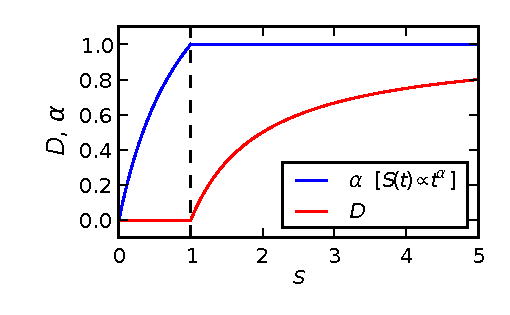
\includegraphics[width=0.45\textwidth]{alexander}
  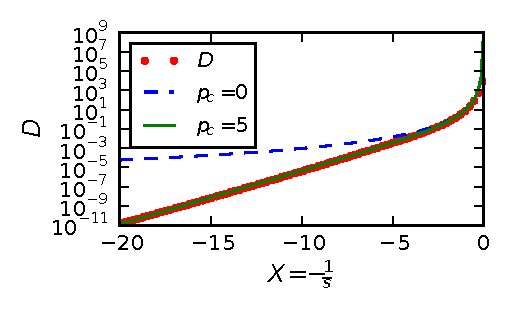
\includegraphics[width=0.45\textwidth]{ERH}
\caption{On the left: theoretical $1d$ chain model. On the right: numerical spectral analysis results vs ERH for $2d$.}
\label{fig:alexander}
\end{figure}

  }





%%%%%%%%%%%%%%%%%%%%%%%%%%%%%%%%%%%%%%%%%%%%%%%%%%%%%%%%%%%%%%%%%%%%%%%%%%%%%%
  \headerbox{Eigenvalue distributions}{name=eigvals,column=1,span=2, below=alexander}{
%%%%%%%%%%%%%%%%%%%%%%%%%%%%%%%%%%%%%%%%%%%%%%%%%%%%%%%%%%%%%%%%%%%%%%%%%%%%%%
%%%%%%%%%%%%%%%%%%5
\begin{figure}[H]
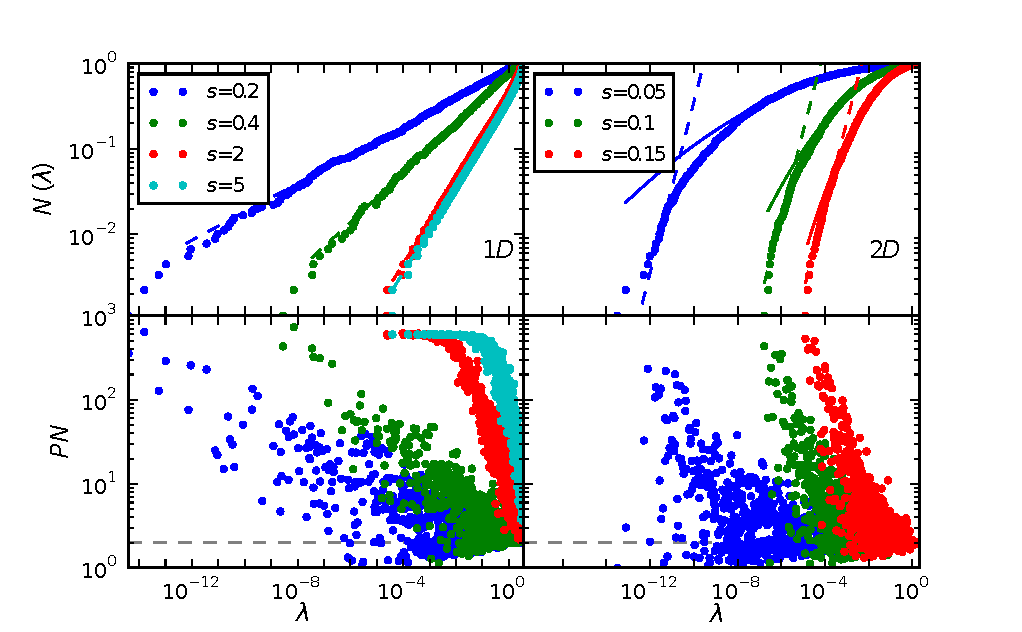
\includegraphics[clip, width=0.95\textwidth]{four_panels}
\caption{ Spectral properties for $1D$ and $2D$. The upper panels show the cumulative density of the eigenmodes, while the lower panels present the participation number of each mode. Modes with high participation numbers are extended and are more important for the long term behaviour. In $1d$ there is a sub diffusive regime with a slope of less than $1/2$, while in $2d$ the low-$\lambda$ slope is always $1$.} \label{fig:exp_2d_D_vs_subD}
\end{figure}
}


%%%%%%%%%%%%%%%%%%%%%%%%%%%%%%%%%%%%%%%%%%%%%%%%%%%%%%%%%%%%%%%%%%%%%%%%%%%%%%
  \headerbox{Banded Lattice Model}{name=banded,column=1,span=2, below=eigvals,above=refs}{
%%%%%%%%%%%%%%%%%%%%%%%%%%%%%%%%%%%%%%%%%%%%%%%%%%%%%%%%%%%%%%%%%%%%%%%%%%%%%%
\begin{figure}[H]
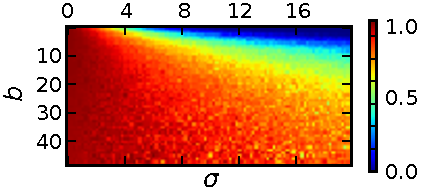
\includegraphics[height=10em]{resnet_new}
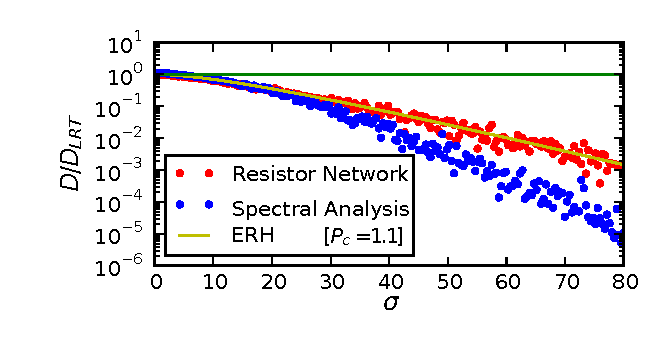
\includegraphics[height=10em]{banded_b10}
\caption{$D/D_{LRT}$. On the left: the resistor network method result, for many values of $b$ and $\sigma$.
On the right: the resistor network method and the spectral analysis results, for $b=10$, together with the ERH approximation.}
\end{figure}

}



\end{poster}

\end{document}
